\ignore{
\begin{figure}[t]
\centering
\includegraphics[width=\columnwidth]{plots/time.pdf}
\caption{off line time consuming of different model size with 5 clusters on with 30 frames length animation.}
\label{fig:time}
\end{figure}
}

\begin{table*}
\newcolumntype{Y}{>{\centering\arraybackslash}X}
\newcommand{\ce}[1]{\multicolumn{1}{c}{#1}}
\caption{Preprocessing times (in seconds) for all combinations of models, motions, and parameter settings.}
\label{tab:preproc}
\begin{center}
\setlength{\tabcolsep}{3.2pt}
\footnotesize
%\small
\begin{tabularx}{\textwidth}{l *{14}{Y}}
\toprule
\multirow{2}*{Model} &
\multicolumn{7}{c}{$\lambda=0.85$} &
\multicolumn{7}{c}{$\lambda=3$} \\
\cmidrule(l{2pt}r{2pt}){2-8}
\cmidrule(l{2pt}r{2pt}){9-15}
& {\emph{A}} & {\emph{B}} & {\emph{C}} & {\emph{D}} & {\emph{E}} & {\emph{F}} & {\emph{joint}} & {\emph{A}} & {\emph{B}} & {\emph{C}} & {\emph{D}} & {\emph{E}} & {\emph{F}} & {\emph{joint}}\\
\cmidrule(l{2pt}r{2pt}){2-8}
\cmidrule(l{2pt}r{2pt}){9-15}
Ganfaul & 420 & 245 & 365 & 204 & 229 & 213 & 2507 & 648 & 248 & 369 & 350 & 286 & 273 & 2445\\
Kachujin &382 & 333 & 320 & 277 & 295 & 189 & 1727 & 395 & 230 & 417 & 248 & 206 & 196 & 2639\\
Maw & 442 & 396 & 604 & 293 & 235 & 284 & 3420 & 558 & 464 & 501 & 433 & 293 & 285 & 3126\\
Nightshade & 384 & 369 & 362 & 495 & 296 & 366 & 2128 & 479 & 245 & 450 & 308 & 221 & 262 & 2282\\
\bottomrule
\end{tabularx}
\bigskip
\end{center}
\vspace*{-1.5ex}
\end{table*}

\begin{figure}[t]
\centering
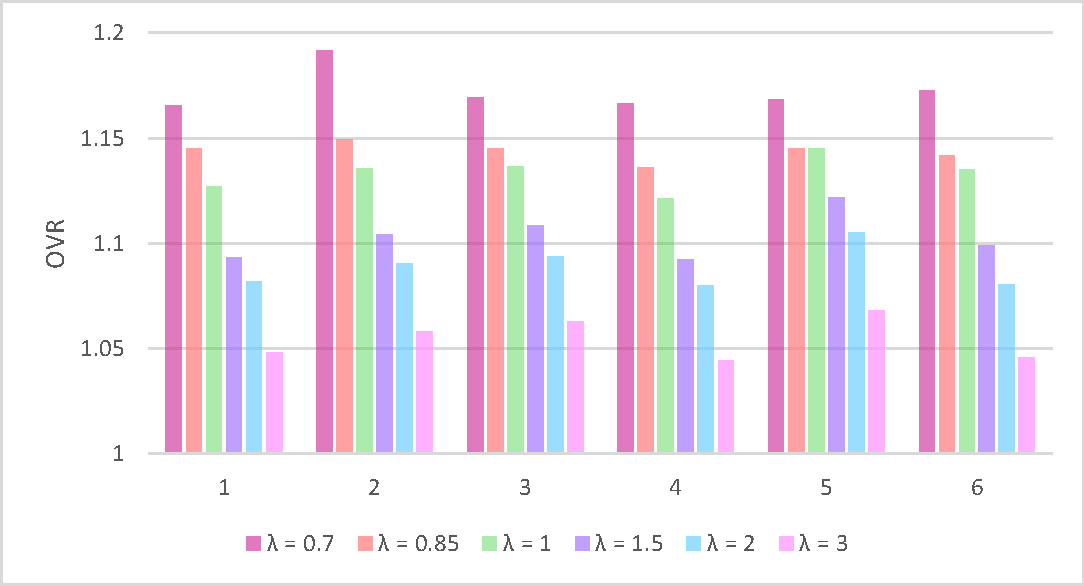
\includegraphics[width = \columnwidth]{plots/alpha.pdf}%
\caption{Adjusting $\lambda$ provides a tradeoff between vertex caching and overdraw, as shown here for the six animations of the Ganfaul model.}
\label{fig:alpha}
\end{figure}

\begin{figure}[t]
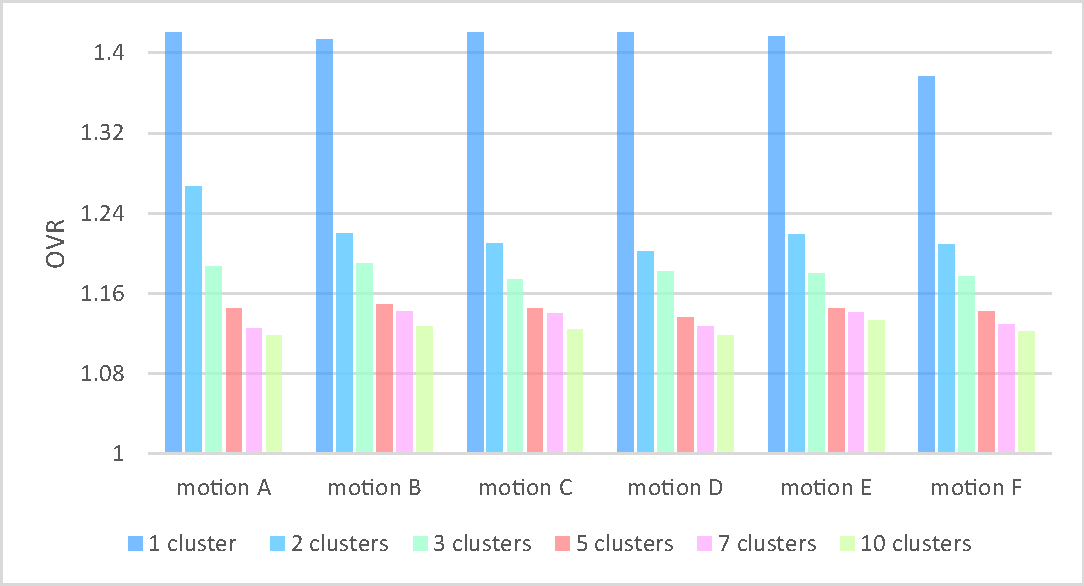
\includegraphics[width=\columnwidth]{plots/GanfaulClusters.pdf}
\caption{The number of clusters trades off memory (one index buffer per cluster) and overdraw, as shown here for the six animations of the Ganfaul model.}
\label{fig:clusters}
\end{figure}

\section{Results}
\label{sec:results}

In this section, we present results of our approach.
Our results use four models undergoing a set of six complex animations
that have between 30 and 70 keyframes.  These are representative of animated characters often found in games
and other real-time applications. Refer to the supplemental video for a demonstration of these animations.
Table~\ref{tab:preproc} shows preprocessing times for creating index buffers for each animation (labeled {\em A-F}), as well as
for a {\em joint} set of buffers that is optimized for all animations. Note that we did not heavily optimize
the preprocessing computation for speed, since this is done offline and only once after modeling. We focused on reducing overdraw for higher runtime performance
on pixel bound scenes.

\ignore{All experiments were conducted
on an Intel\textsuperscript{\textregistered}
Xeon\textsuperscript{\textregistered} 2.27GHz E5520 
CPU with 12GB of RAM and an AMD
Radeon HD 6970 GPU.}

\paragraph{Choice of $\boldsymbol\lambda$} As mentioned earlier, rendering time has been shown to be
directly proportional to ACMR for vertex-bound scenes, and OVR for pixel-bound
scenes~\citep{Sander07}. The algorithm trades off these objectives by controlling the
desired ACMR through the $\lambda$ parameter. Figure~\ref{fig:alpha} shows how the overdraw ratio is affected by the choice
of $\lambda$. We have found that setting $\lambda$ in the range of $0.75-0.95$ provides a
good balance between ACMR and OVR objectives for our animated scenes. For the remaining results in this paper, we use $\lambda=0.85$.
In addition, we also provide results for $\lambda=3$, which is the
extreme case where vertex cache performance is not taken into account and results
are solely optimized for reduced overdraw.

\paragraph{Choice of number of clusters} Figure~\ref{fig:clusters} shows results for different number of clusters for the Ganfaul model.
Increasing the number of clusters reduces overdraw at the expense of memory to store the additional index
buffers. We have found that using more than five clusters only yields modest ovedraw reduction for the models and animations that we tested. Thus,
for the remaining results in the paper, we use five clusters.

\paragraph{Overall results} Table~\ref{tab:stats} shows the statistics of each of our four models. Results are averaged over all keyframes and over a set of 300 random viewpoints within a radius three times that of the object's bounding sphere. The {\em original} results use a single index buffer that is optimized solely for reduced ACMR. It has a low memory footprint since it only requires one buffer, however it results in an order with high overdraw. The {\em tipsify} results use the state-of-the-art algorithm for static scenes described in ~\cite{Sander07} applied to {\em each individual frame}. It reduces overdraw significantly, but requires between 30-70 index buffers, depending on the animation, making its direct use impractical. Our {\em single} set of results uses five clusters for each single animation, thus requiring only five index buffers per animation and our cluster-based approach further reduces overdraw significantly for both $\lambda = 0.85$ and $\lambda = 3$. Our {\em joint} set of results optimize for the same five clusters for all frames in {\em all animations}. It therefore does slightly worse than the single animation results. As described earlier, the choice of $\lambda$ affects the resulting ACMR. With $\lambda = 0.85$, ACMR is kept under 0.9, while for $\lambda = 3$, the order is solely optimized for overdraw, thus ACMR is significantly sacrificed to achieve this additional reduction in overdraw. Figure~\ref{fig:results} further breaks down the results for each animation (labeled {\em motion A-F}). Note that the improvements of our algorithm are consistent over a variety of different character animations and brings the overdraw ratio very close to the optimal value of 1.

\paragraph{Rendering times} We conducted experiments to verify the dependency between OVR and rendering time~\citep{Sander07}. We used the Kachujin model with $\alpha=0.85$ in a heavily pixel bound scene. We noticed the improvement in rendering time closely matched the improvement in OVR ($\sim$18-20\%). With an inexpensive shader that simply outputs the color, the improvement was less significant ($\sim$10\%).

\begin{table*}
\newcolumntype{Y}{>{\centering\arraybackslash}X}
\newcommand{\ce}[1]{\multicolumn{1}{c}{#1}}
\caption{Average cache miss ratio (ACMR) and overdraw ratio (OVR) results for several character animations. We contrast our method with a triangle order that only considers vertex caching (original), and with the approach for static meshes of \cite{Sander07}, which applies the algorithm to each frame independently, resulting in 30-70 index buffers per animation (tipsify). We present our results using a separate set of five index buffers per motion (single) and with a joint set of five index buffers for all motions combined (joint).}
\label{tab:stats}
\begin{center}
\setlength{\tabcolsep}{3.2pt}
\footnotesize
%\small
\begin{tabularx}{\textwidth}{lr *{14}{Y}}
\toprule
\multirow{2}*{Model} &
\multirow{2}*{\# tris} &
\multicolumn{2}{c}{Original} &
\multicolumn{2}{c}{Tipsify ($\lambda=0.85$)} &
\multicolumn{2}{c}{Tipsify ($\lambda=3$)} &
\multicolumn{2}{c}{Single ($\lambda=0.85$)} &
\multicolumn{2}{c}{Single ($\lambda=3$)} &
\multicolumn{2}{c}{Joint ($\lambda=0.85$)} &
\multicolumn{2}{c}{Joint ($\lambda=3$)} \\
\cmidrule(l{2pt}r{2pt}){3-4}
\cmidrule(l{2pt}r{2pt}){5-6}
\cmidrule(l{2pt}r{2pt}){7-8}
\cmidrule(l{2pt}r{2pt}){9-10}
\cmidrule(l{2pt}r{2pt}){11-12}
\cmidrule(l{2pt}r{2pt}){13-14}
\cmidrule(l{2pt}r{2pt}){15-16}
& & {\emph{ACMR}} & {\emph{OVR}} & {\emph{ACMR}} & {\emph{OVR}} & {\emph{ACMR}} & {\emph{OVR}} & {\emph{ACMR}} & {\emph{OVR}} & {\emph{ACMR}} & \ce{\emph{OVR}} & {\emph{ACMR}} & \ce{\emph{OVR}} & {\emph{ACMR}} & \ce{\emph{OVR}}\\
\midrule
%Ganfaul & 13,801 & 0.676 & 1.351 & 0.869 & 1.296 & 2.939 & 1.214 & 0.860 & 1.139 & 2.715 & 1.054\\
%Kachujin & 12,610 & 0.645 & 1.308 & 0.903 & 1.178 & 2.896 & 1.120 & 0.891 & 1.076 & 2.619 & 1.024\\
%Maw & 13,908 & 0.619 & 1.395 & 0.879 & 1.255 & 2.918 & 1.165 & 0.860 & 1.097 &  2.694& 1.036\\
%Nightshade & 12,996 & 0.656 & 1.309 & 0.862 & 1.178 & 2.930 & 1.114 & 0.854 & 1.067 & 2.640 & 1.022\\
Ganfaul & 13,801 & 0.676 & 1.355 & 0.869 & 1.298 & 2.939 & 1.213 & 0.862 & 1.144 & 2.715 & 1.055 & 0.860 & 1.144 & 2.684 & 1.064\\
Kachujin & 12,610 & 0.645 & 1.310 & 0.903 & 1.172 & 2.896 & 1.122 & 0.891 & 1.068 & 2.617 & 1.027 & 0.887 & 1.102 & 2.570 & 1.030 \\
Maw & 13,908 & 0.619 & 1.380 & 0.879 & 1.253 & 2.918 & 1.166 & 0.860 & 1.101 &  2.696 & 1.038 & 0.859 & 1.109 & 2.675 & 1.044 \\
Nightshade & 12,996 & 0.656 & 1.302 & 0.862 & 1.172 & 2.930 & 1.112 & 0.854 & 1.068 & 2.643 & 1.024 & 0.854 & 1.071 & 2.612 & 1.027 \\
\bottomrule
\end{tabularx}
\bigskip
\end{center}
\vspace*{-1.5ex}
\end{table*}

\begin{figure*}[t]
\centering
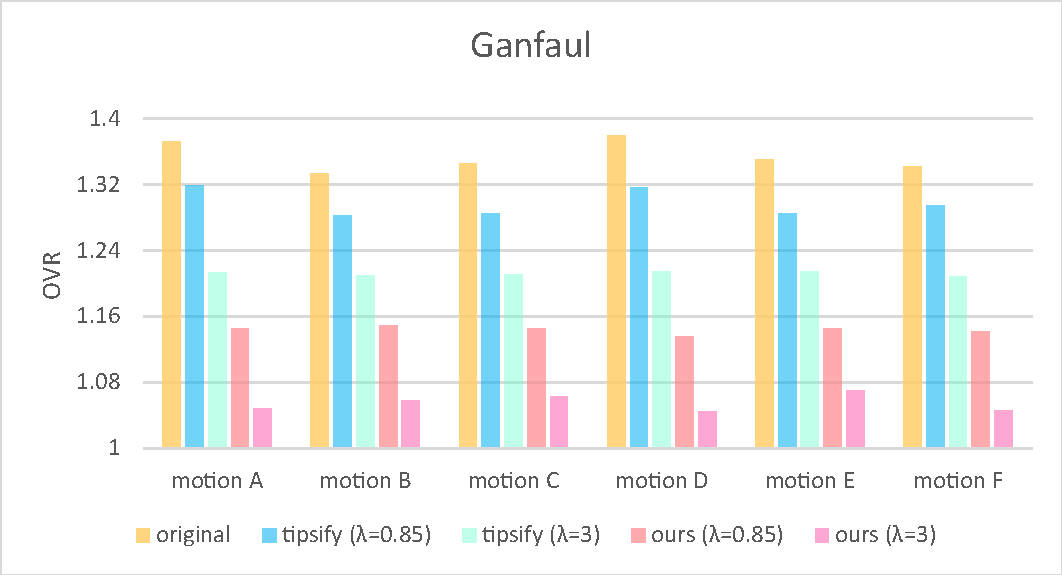
\includegraphics[width=.49\textwidth]{plots/GanfaulRatio.pdf}
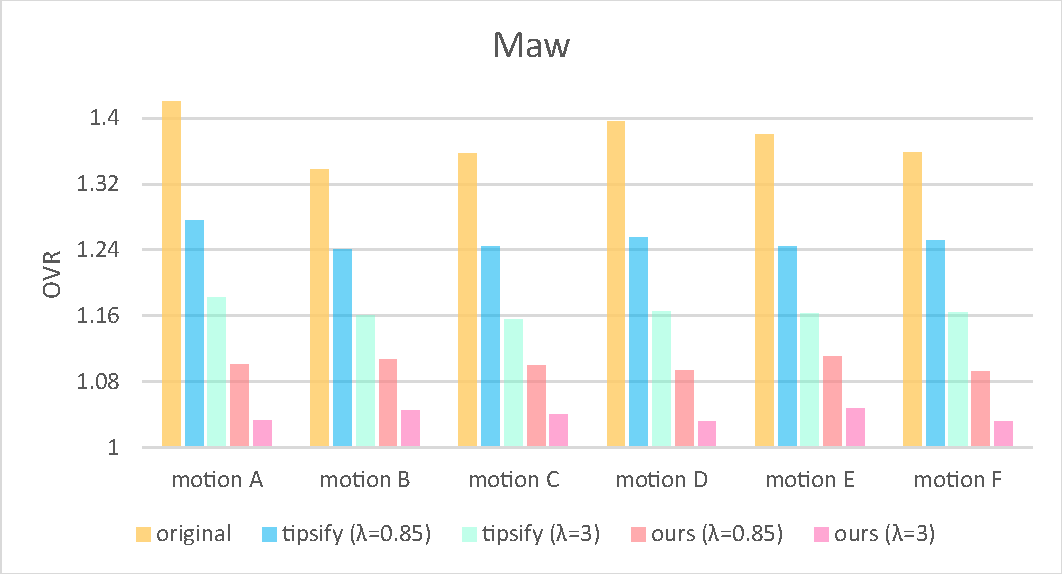
\includegraphics[width=.49\textwidth]{plots/MawRatio.pdf}
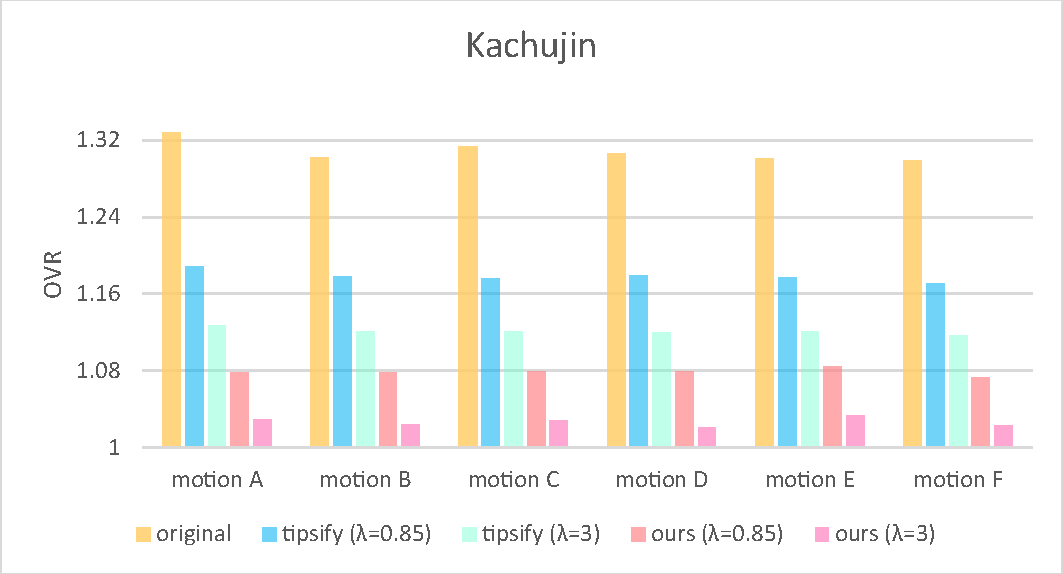
\includegraphics[width=.49\textwidth]{plots/KachujinRatio.pdf}
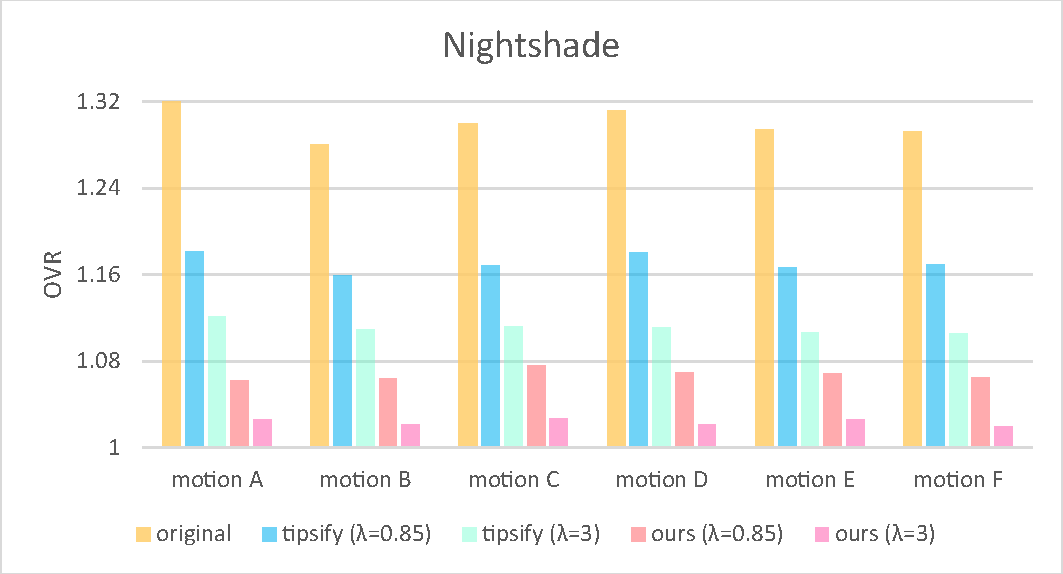
\includegraphics[width=.49\textwidth]{plots/NightshadeRatio.pdf}
\caption{Average overdraw ratio for different animations of the four models from Table~\ref{tab:stats}.}
\label{fig:results}
\end{figure*}

\ignore{??
Patch position is area-weighted
Normalize center position of frame to avoid giving higher distance weights to some frames in the presence of motion

??Using multiple buffers is what makes our overdraw better. tipsify restricted to one per frame
}







